We now describe our experimental setup. We use this setup to conduct two case studies that demonstrate the type of research that our memory system models enable.

\subsection{Target Designs}

\begin{table}[htbp]
\begin{center}
\resizebox{0.85\linewidth}{!}{%
\begin{tabular}{|r|c c|}
\hline
 & \textbf{Rocket} & \textbf{BOOM-2w} \\
\hline
\textit{Fetch-width} & 1 & 2 \\
\textit{Issue-width} & 1 & 3 \\
\textit{Issue slots} & - & 16 \\
\textit{ROB size} & - & 48 \\
\textit{Ld/St entries} & - & 16/16 \\
\textit{Physical registers} & 32(int)/32(fp) & 110 \\
\textit{Branch predictor} & - & tage \\
\textit{MSHR entries} & 2 & 6 \\
\textit{L1 I\$ and D\$} & \multicolumn{2}{c|}{16KiB / 16KiB} \\
\textit{ITLB and DTLB reaches} & \multicolumn{2}{c|}{128KiB / 128KiB} \\
\hline
\end{tabular}}
\end{center}
\caption{Processor Parameters}
\label{tbl:target}
\end{table}%

Our memory model can be simulated alongside any FPGA-model that presents a
host-decoupled AXI4 master port -- this includes RTL transformed from source,
or manually written models that conform to RAMP-style host-decoupling.

To demonstrate this flexibility, we evaluate two microarchitecturally different processors, both
of which leverage the open-source Rocket-Chip SoC generator~\cite{rocketchip}. The first
processor is Rocket, a 5-stage single-issue in-order core, and the second processor is BOOM, a
superscalar out-of-order processor~\cite{boom}. Both processors implement the 64-bit scalar
RISC-V ISA~\cite{Waterman:EECS-2016-118, Waterman:EECS-2016-161}, which includes support for
atomics, IEEE 754-2008 floating-point, and page-based virtual memory (RV64IMAFD).
Table~\ref{tbl:target} lists the selected configurations of the target processors. Note that
BOOM-2w roughly approximates the configuration of the ARM Cortex-A9 processor.

The target designs are automatically transformed into the FPGA performance
simulators using the FIRRTL compiler passes described in Section~\ref{sec:infrastructure}.

\subsection{System Setup}

We performed our experiments on a small cluster of Xilinx ZC706 development boards, which feature
a Zynq XC7Z045 FPGA (hardened ARM A9, Kintex-7 fabric architecture with 19.1Mb of BRAM and 350K
logic cells) with 512MiB (ARM-side) + 8GiB (fabric-side) of on-board DRAM.

Figure~\ref{fig:platform} describes how the target systems are mapped to the host platform. A
simulation \textit{master} (or \emph{driver}) runs on the embedded ARM core. It is responsible
for initializing stateful simulation components, regulating simulation time\footnote{Simulation advances via dataflow \cite{APortNetworks}. The master ``regulates''
simulation time by controlling the flow of tokens to the target.}, and periodically profiling
target behavior. All fabric-hosted stateful simulation components expose an AXI4-lite interface
connected to an AXI4 master presented by the ARM core. Finally, the master also hosts an instance
of the RISC-V front-end server (\texttt{fesvr}), which manages a tether used to virtualize console
IO connected to the target hosted on the FPGA.

\begin{table*}
\centering
	\begin{tabular}{|c|S[table-format=5]|c|S[table-format=5]|c|S[table-format=5]|c|S[table-format=5]|c|}
	\hline
	& \multicolumn{2}{c|}{\textbf{Latency-Bandwidth Pipe}} & \multicolumn{2}{c|}{\textbf{Bank Conflict Model}} & \multicolumn{2}{c|}{\textbf{FIFO MAS}} & \multicolumn{2}{c|}{\textbf{FR-FCFS}} \\
	\hline
	\textbf{Resource} & \textbf{Utilization} & \textbf{\%} & \textbf{Utilization} & \textbf{\%} & \textbf{Utilization} & \textbf{\%} & \textbf{Utilization} & \textbf{\%} \\
	\hline
	\textit{LUT} & 3586 & 1.6 & 4170 & 1.9 & 3812 & 1.7 & 6822 & 3.1 \\
	\textit{LUTRAM} & 651 & 0.9 & 607 & 0.8 & 655 & 0.9 & 693 & 1.0 \\
	\textit{FF} & 3146 & 0.7 & 3929 & 0.9 & 3426 & 0.8 & 5282 & 1.2 \\
	\textit{BRAM} & 11 & 2.0 & 11 & 2.0 & 11 & 2.0 & 11 & 2.0 \\
	\hline
	\end{tabular}

\caption{Resource utilization of various memory system models for Xilinx zc706 FPGA}
\label{tbl:utilization}
\end{table*}

Table~\ref{tbl:utilization} shows the resource utilization of various memory system models
developed in this paper. Complex models such as FR-FCFS consumes more resources than simpler
models like Latency-Bandwidth Pipe, but in general, their overhead is very small for FPGAs
used for the evaluations.

\subsection{System Software}

\begin{figure}
	\centering
	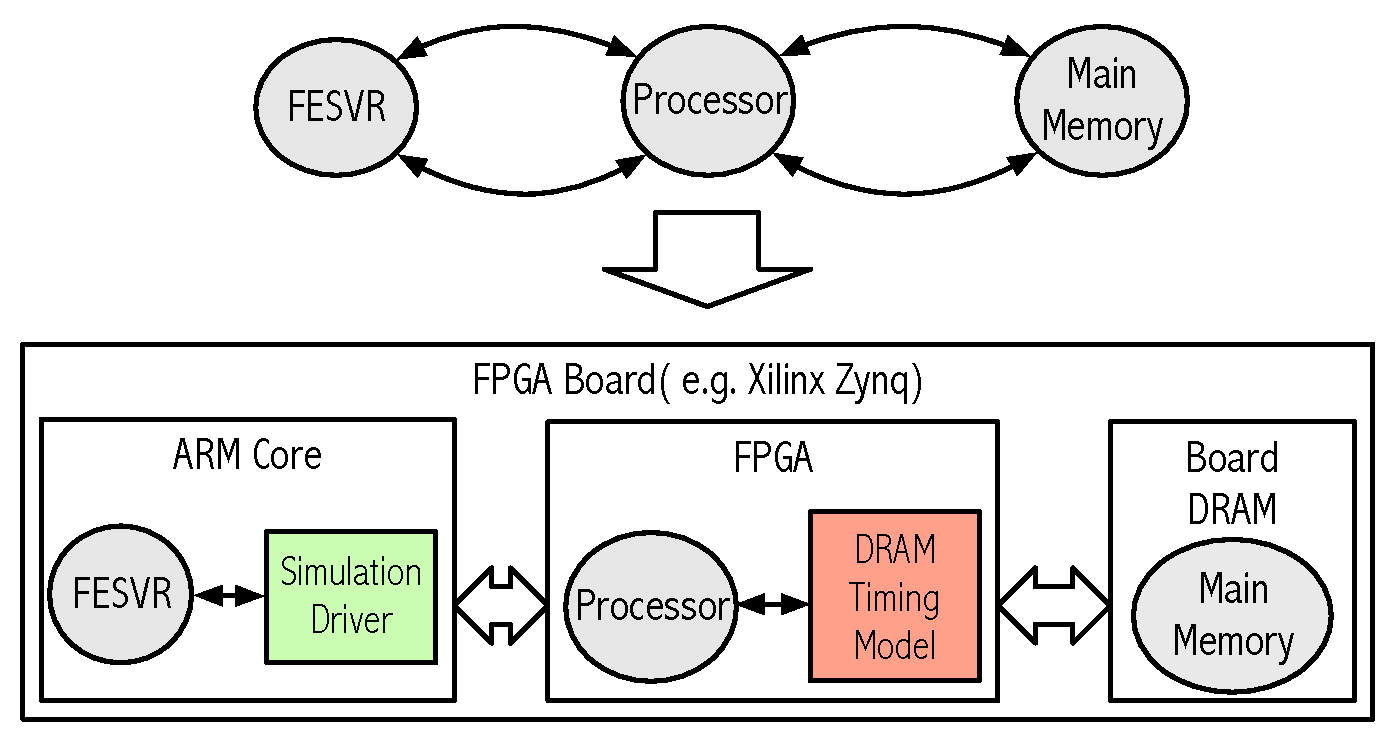
\includegraphics[width=\columnwidth]{figures/platform.pdf}
	\caption{Mapping the target design to the host platform}
	\label{fig:platform}
\end{figure}

Unless otherwise stated, all benchmarks were run on Linux kernel version 4.6.2. For each benchmark, we built a minimal BusyBox image and included all required files for a given benchmark within an initramfs. For complex workloads, such as our JVM, we built library dependencies using the Yocto (\texttt{riscv-poky}) Linux distribution generator.


\subsection{Workloads}

The goal of our evaluation is to demonstrate that our platform allows us to perform high-fidelity
experiments involving realistic software applications without sampling. We therefore chose two
non-trivial benchmark suites, the SPEC 2006 CPU benchmarks~\cite{spec_cpu_2006} and the DaCapo
benchmarks~\cite{dacapo}.

%\subsubsection{ccbench $\mu$benchmarks}
%\TODO{Chris?}

\subsubsection{SPECint2006 Benchmarks} The SPECint2006 benchmarks are widely used by computer
architects to validate their designs. However, evaluations using microarchitectural cycle-level
software simulators typically do not run the entire benchmarks, due to their non-trivial lengths
of execution~\cite{simpoints, smarts}.

Table~\ref{tbl:spec} shows the dynamic instruction counts and the cache and TLB misses per 1000
instructions~(MPKI) for each benchmark compiled by \textit{riscv-gcc} and executed with test inputs. Note that it takes at
least 8 days to run the whole set of benchmarks with test inputs on a single instance of a
very fast microarchitectural cycle-accurate software simulator (400~KIPS)~\cite{marssx86}.

\begin{table}[t]
	\begin{center}
	\begin{subtable}[t]{0.7\columnwidth}
		\begin{tabular}{|c|S[table-format=3.1]|S[table-format=3.1]|}
		\hline
		\textbf{Benchmarks} & \textbf{Instructions~(B)} & \textbf{MPKI} \\
		\hline
		\textit{400.perlbench} & 2.6 & 49.5 \\
		\textit{401.bzip2} & 34.4 & 27.5 \\
		\textit{403.gcc} & 5.4 & 37.2 \\
		\textit{429.mcf} & 3.5 & 274.6\\
		\textit{445.gobmk} & 66.4 & 36.4 \\
		\textit{456.hmmer} & 16.5 & 4.3 \\
		\textit{458.sjeng} & 18.9 & 23.1 \\
		\textit{462.libquantum} & 0.3 & 32.0 \\
		\textit{464.h264ref} & 104.2 & 7.5 \\
		\textit{471.omnetpp} & 1.9 & 61.0 \\
		\textit{473.astar} & 22.8 & 45.8 \\
		\textit{483.xalancbmk} & 0.4 & 64.3 \\ 
		\hline
		\end{tabular}
		\caption{Test Input}
		\label{tbl:spec_test}
		\vspace{0.2cm}
	\end{subtable}
	\begin{subtable}[t]{0.7\columnwidth}
		\begin{tabular}{|c|c|c|}
		\hline
		\textbf{Benchmarks} & \textbf{Instructions~(B)} & \textbf{MPKI} \\
		\hline
		\textit{403.gcc} & 1366.5 & 54.2 \\
		\hline
		\end{tabular}
		\caption{Reference Input}
		\label{tbl:spec_ref}
	\end{subtable}
	\end{center}
	\caption{Dynamic instruction counts and MPKI for the SPECint2006 benchmarks}
	\label{tbl:spec}
\end{table}

\subsubsection{DaCapo Benchmarks}

\begin{table}
\begin{center}
\resizebox{0.7\linewidth}{!}{%
	\begin{tabular}{|c|S[table-format=3.1]|S[table-format=2.1]|}
	\hline
	\textbf{Benchmarks} & \textbf{Instructions~(B)} & \textbf{MPKI} \\
	\hline
	\textit{avrora} & 216.5 & 51.2 \\
	\textit{luindex} & 72.5 & 30.5 \\
	\textit{lusearch} & 131.5 & 34.1 \\
	\textit{pmd} & 109.6 & 34.1 \\
	\textit{sunflow} & 124.5 & 41.6 \\
	\textit{xalan} & 152.9 & 37.9 \\
	\hline
	\end{tabular}
}%
\end{center}
\caption{Dynamic instruction counts and MPKI for the DaCapo benchmarks with the ``small'' input size}
\label{tbl:dacapo}
\end{table}

To demonstrate how our platform enables studies that are difficult to perform in existing FPGA-based simulators and cycle-accurate software simulators, we run the DaCapo benchmarks on JikesRVM, a research Java Virtual Machine that is widely used in managed-language research.

The DaCapo benchmarks are widely used Java benchmarks that represent full Java applications, including the Lucene search engine and a raytracer. We use version 9.12 of the benchmark suite and exclude the benchmarks that do not run on recent versions of JikesRVM. Specifically, we run \emph{avrora}, \emph{luindex}, \emph{lusearch}, \emph{pmd}, \emph{sunflow} and \emph{xalan}.

For each benchmark, we ran one full pass of the ``small'' input size, accounting for both class loading and Just-in-Time compilation. We believe that this gives a comprehensive and realistic view of the full execution of a Java program. Figure~\ref{tbl:dacapo} shows the dynamic instruction counts and MPKI for each benchmark with the ``small'' input size.

JikesRVM is configured to use the \emph{MarkSweep} garbage collector and the default settings. MarkSweep is a non-relocating Mark \& Sweep Garbage Collector with a segregated free-list allocator (meaning that it maintains a number of free lists for different size classes of objects, with a shared pool of pages that can be acquired and released by these free lists).
